\newcommand\tab[1][1cm]{\hspace*{#1}}
\begin{enumerate}

\item U \texttt{Windows} okružeju pokrenuti \texttt{DE1SoC\_SystemBuilder} [dostupan gde?]
\item Izabrati konfiguraciju kao na slici \ref{slika:sb} i izabrati Generate\\
\begin{figure}[h!]
\centering
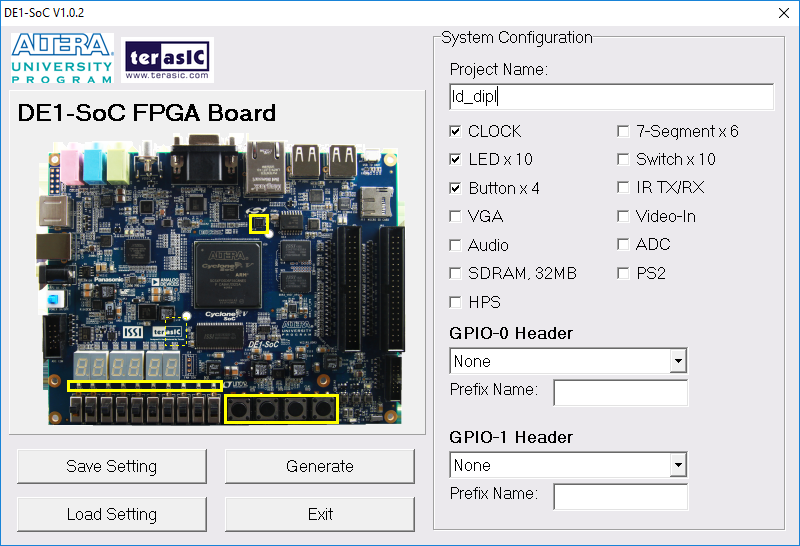
\includegraphics[scale=0.8]{img/DE1SoC_SystemBuilder.png}
\caption{Podešavanja \texttt{DE1\_Soc Bulder}-a}
\label{slika:sb}
\end{figure}\\

Od genersianih fajlova značajni su:
\begin{itemize}
\item .qpf - projektni fajl za Quartus
\item .qsf - skripta za podešavanje pinova
\item .sdc - skripta za podešavanje takta
\item .v - Verilog HDL fajl
\end{itemize}
\item  Izbristati \texttt{ld\_dipl.v} fajl (kasnije će biti napravljen \texttt{ld\_dipl.vhd} fajl za VHDL)
\item  Kopirati fajlove u \texttt{Ubuntu} u radni folder \texttt{$\sim$/ld\_dipl/hw/}
\item  Pokrenuti \texttt{Quartus (Quartus Prime 18.0) Lite Edition}
\item  Otvoriti projekat komandom \texttt{File > Open Project...} i izabrati \texttt{$\sim$/ld\_dipl/hw/ld\_dipl.qpf}
\item U prozoru \texttt{Tasks} izabrati \texttt{Edit Settings}, u novom prozoru pod \texttt{Timing Analyser} ispod teksta \texttt{SDC files to include in the project} klikom na dugme '...' izabrati fajl \texttt{ld\_dipl.sdc}
\item  Pokrenuti \texttt{Platform Designer (Tools > Platform Designer)}
\item  Iz prozora \texttt{IP Catalog} izabrati \texttt{Processors and Peripherials} \texttt{> Hard Processor Systems >} \texttt{ArriaV/Cyclone V Hard Processor System}
\item  Ovim se otvara meni za podešavanje HPS modula
\item  Pod tabom FPGA interfaces izvršiti sledeće izmene:
\begin{itemize}
\item	U opštim podešavanjima isključiti opciju Enable MPU standbz and event signals
\item	U podešavanjima AXI Bridges podesiti FPGA-to-HPS interface i HPS-to-FPGA interface na unused, a Lightweight HPS-to-FPGA na 32-biti
\item	U podešavanjima FPGA-to-HPS SDRAM Interface izabrati \texttt{f2h\_sdram0} i zatim isključiti pritiskom na dugme '-'
\item	U podešavanjima Interrupts uključiti opciju Enable FPGA-to-HPS interrupts
\end{itemize}
\item  Pod tabom Peripherial Pins izvršiti sledeće izmene
\begin{itemize}
\item	U podešavanjima SD/MMC Controller postaviti SDIO pin na HPS I/O Set 0 i SDIO mode na 4-bit Data
\item	U podešavanjima UART Controllers postaviti UART0 pin na HPS I/O Set 0 i UART mode na No Flow Control
\end{itemize}
	\begin{figure}[h!]
	\centering
	\textit{U ovom tabu je za potrebe nekog drugog projekta moguce uključiti ostale periferije: CAN Controller, Ethernet Media Access Controller, I2C Controller, SPI Controller, QSPI Flash Controller, NAND Flash Controller, Trace Port Intefrace Unit, GPIO za podesavanja pogledati []}
	\end{figure}
\item  Pod tabom HPS Clocks ostaviti podešavanja na podrazumevanim vrednostima
\item  Pod tabom SDRAM podesiti:
\begin{itemize}
\item	SDRAM Protocol: DDR3
\item	PHY Settings:
\begin{itemize}
\item		Clocks:
\begin{itemize}
\item			Memory clock frequency: 400.0 MHz
\item			PLL reference clock frequency: 25.0 MHz
\end{itemize}
\item		Advanced PHY Settings:
\begin{itemize}
\item			Supply Voltage: 1.5V DDR3
\end{itemize}
\end{itemize}
\item	Memory Parameters:
\begin{itemize}
\item		Memory vendor: Other
\item		Memory device speed grade: 800.0 MHz
\item		Total interface width: 32
\item		Number of chip select/depth expansion: 1
\item		Number of clocks: 1
\item		Row address width: 15
\item		Column address width: 10
\item		Bank-address width: 3
\item		Uključiti DM pins
\item		Uključiti \texttt{DQS\#}
\item		Memory Initialization Options:
\begin{itemize}
\item			Mirror Addressing: 1 per chip select: 0
\item			Burst Length: Burst chop 4 or 8 (on the fly)
\item			Read Burst Type: Sequential
\item			DLL precharge power down: DLL off
\item			Memory CAS latency setting: 11
\item			Output drive strength setting: RZQ/7
\item			ODT Rtt nominal value: RZQ/4
\item			Auto selfrefresh method: Manual
\item			Selfrefresh temperature: Normal
\item			Memory write CAS latency setting: 8
\item			Dynamic ODT (\texttt{Rtt\_WR}) value: RZQ/4
\end{itemize}
\end{itemize}
\item	Memory Timing:
\begin{itemize}
\item		tIS (base): 180 ps
\item		tIH (base): 140 ps
\item		tDS (base): 30 ps
\item		tDH (base): 65 ps
\item		tDQSQ: 125 ps
\item		tQH: 0.38 cycles
\item		tDQSCK: 255 ps
\item		tDQSS: 0.25 cycles
\item		tQSH: 0.4 cycles
\item		tDSH: 0.2 cycles
\item		tDSS: 0.2 cycles
\item		tINIT: 500 us
\item		tMRD: 4 cycles
\item		tRAS: 35.0 ns
\item		tRCD: 13.75 ns
\item		tRP: 13.75 ns
\item		tREFI: 7.8 us
\item		tRFC: 260.0 ns
\item		tWR: 15.0 ns
\item		tWTR: 4 cycles
\item		tFAW: 30.0 ns
\item		tRRD: 7.5 ns
\item		tRTP: 7.5 ns
\end{itemize}
\item	Board Settings:
\begin{itemize}
\item		Setup and Hold Derating:
\begin{itemize}
\item			Use Altera's default settings
\end{itemize}
\item		Channel Signal Integrity:
\begin{itemize}
\item			Use Altera's default settings
\end{itemize}
\item		Board Skews:
\begin{itemize}
\item			Maximum CK delay to DIMM/device: 0.03 ns
\item			Maximum DQS delay to DIMM/device: 0.02 ns
\item			Minimum delay difference between CK and DQS: 0.06 ns
\item			Maximum delay difference between CK and DQS: 0.12 ns
\item			Maximum skew within DQS group: 0.01 ns
\item			Maximum skew between DQS groups: 0.06 ns
\item			Average delay difference between DQ and DQS: 0.05 ns
\item			Maximum skew within address and command bus: 0.02 ns
\item			Average delay difference between address and command and CK: 0.01 ns
\end{itemize}
\end{itemize}
\end{itemize}
Ovim su podešavanja HPS modula završena, izabrati Finish
\item  Duplim klikom u Export koloni eksportovati signale memory pod imenom \texttt{hps\_0\_ddr} i signale \texttt{hps\_io} pod imenom \texttt{hps\_0\_io}.
\item  Povezati HPS sa izvorom takta kao što je prikazano na slici \ref{slika:q1}
\begin{figure}[h!]
\centering
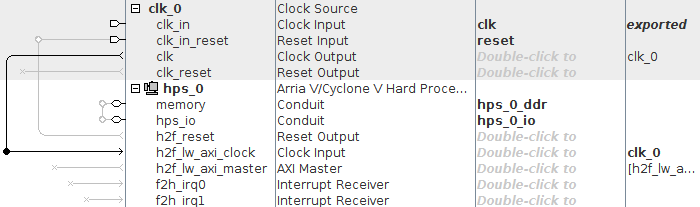
\includegraphics[scale=0.9]{img/quartus1.png}
\caption{Povezivanje HPS i takt signala}
\label{slika:q1}
\end{figure}
\item  Iz prozora \texttt{IP Catalog} izabrati \texttt{Processors and Peripherials > Peripherials > PIO (Parallel I/O) Intel FPGA IP}. Ovim se otvara meni za podešavanje \texttt{PIO IP} bloka
\item  U podešavnjima \texttt{PIO IP} bloka pod Basic Settings postaviti \texttt{Width: 8} i \texttt{Direction: Output}
\item  Preimenovati \texttt{PIO} blok u \texttt{leds\_0}. Duplim klikom u \texttt{Export} koloni eksportovati signale \texttt{external\_connection} i podesiti ime \texttt{leds\_0\_external\_connection}.
\item  Povezati \texttt{leds\_0} blok sa izvorom takta i resetom, zatim povezati Avalon Memory Mapped Slave pod imenom \texttt{s1} sa \texttt{hps\_0} interfejsom \texttt{h2f\_lw\_axi\_master}, kao što je prikazano na slici \ref{slika:q2}
\begin{figure}[h!]
\centering
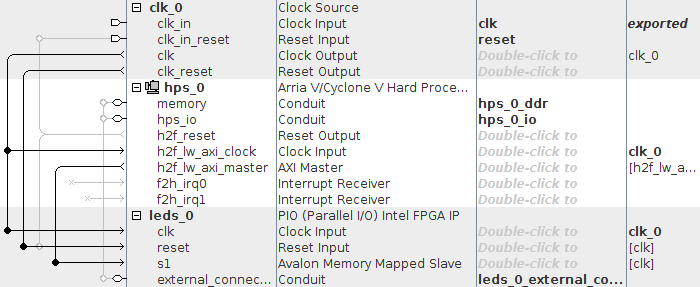
\includegraphics[scale=0.9]{img/quartus2.png}
\caption{Povezivanje \texttt{leds\_0} bloka}
\label{slika:q2}
\end{figure}
\item  Ponovo iz prozora \texttt{IP Catalog} izabrati\texttt{ Processors and Peripherials > Peripherials > PIO (Parallel I/O) Intel FPGA IP}. Ovim se otvara meni za podesavanje \texttt{PIO IP} bloka
\item  U podešavnjima \texttt{PIO IP} bloka pod \texttt{Basic Settings} postaviti \texttt{Width: 8}, \texttt{Direction: Input}.
\item  U podešavanjima \texttt{PIO IP} bloka pod Edge capture register uključiti opciju \texttt{Synchronously capture, Edge Type} podesiti na \texttt{ANY}, i uključiti \texttt{bit-clearing for edge capture register}.
\item  U podešavanjima \texttt{PIO IP} bloka pod Interrupt uključiti opciju \texttt{Generate IRQ} i izabrati \texttt{IRQ Type: EDGE}
\item  Preimenovati \texttt{PIO} blok u \texttt{keys\_0}. Duplim klikom u \texttt{Export} koloni eksportovati signale \texttt{external\_connection} i podesiti ime \texttt{keys\_0\_external\_connection}.
\item  Povezati \texttt{keys\_0} blok sa izvorom takta i resetom, zatim povezati Avalon Memory Mapped Slave pod imenom \texttt{s1} sa \texttt{hps\_0} interfejsom  \texttt{h2f\_lw\_axi\_master} i na kraju povezati \texttt{irq} signal na \texttt{f2h\_irq0} interfejs \texttt{hps\_0} bloka, kao što je prikazano na slici \ref{slika:q3}
\begin{figure}[h!]
\centering
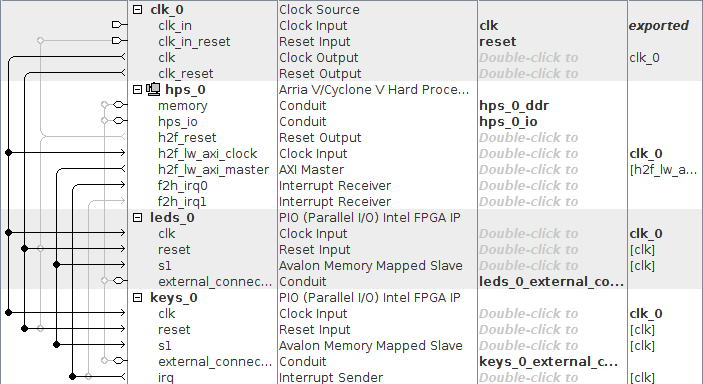
\includegraphics[scale=0.9]{img/quartus3.png}
\caption{Povezivanje \texttt{keys\_0} bloka}
\label{slika:q3}
\end{figure}
\item  Duplim klikom u koloni \texttt{Base} podesiti adresu porta \texttt{s1} bloka \texttt{leds\_0} i porta \texttt{s1} bloka \texttt{keys\_0} kao na tabeli 1.
\item  Sačuvati \texttt{Platform Designer} projekat izborom \texttt{File > Save} i sačuvati ga pod imenom \texttt{ld\_dipl\_system.qsys}
\item  Trebalo bi da se pojavi obaveštenje \texttt{Save System: completed successfully}. Zatim odabrati iz menija \texttt{Generate > Generate HDL... }U novom prozoru podesiti \texttt{Create HDL design files for synthesis: VHDL} i isključiti opciju \texttt{Crete block symbol file (.bsf)}. Pokrenuti generisanje klikom na \texttt{Generate}. Proces bi trebalo da se završi bez grešaka ali može imati upozorenja.
\item  Zatvoriti \texttt{Platform Designer}. U prozoru \texttt{Quartus}-a izabrati \texttt{Project > Add/Remove Files in Project...} i u meniju klikom na '...' izabrati fajl \texttt{ld\_dipl\_system/synthesis/ld\_dipl\_system.qip}.
\item  Izabrati \texttt{File > New VHDL File} i novi fajl nazvati \texttt{ld\_dipl.vhd}. Pod \texttt{Project Navigator > Files} desnim klikom na \texttt{ld\_dipl.vhd} izabrati \texttt{Set as Top-Level Entity}.
\item  U ovom fajlu je potrebno instancirati HPS komponentu iz \texttt{Platform Designer}-a. Potrebno je ručno napiati ovaj fajl (primer za ovaj rad dat je u dodatku. Takođe među generisanim fajovima nalazi se deklaracija komponente \texttt{ld\_dipl\_system} koja može biti od pomoći (fajl \texttt{$\sim$/ld\_dipl/hw/ld\_dipl\_system/ld\_dipl\_system.cmp}).
\item  Izabrati \texttt{Processing > Start > Start Analysis and Synthesis}
\item  Izabrati \texttt{Tools > Tcl Scripts...}\\
\begin{figure}[h!]
\centering
\textbf{Važno: Prozor koji se otvori mora da izgleda upravo kao na slici \ref{slika:tcl} (generisani fajlovi ne smeju biti duplirani). Ukoliko su fajlovi duplirani neophodno je zatvoriti \texttt{Quartus} i pokrenuti ponovo. Neke verzije \texttt{Quartus}-a imaju ovu grešku pri detekciji \texttt{tcl} skripti.}\\
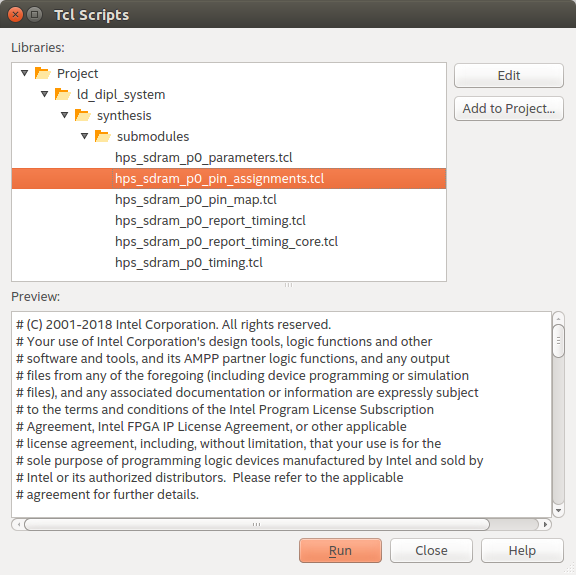
\includegraphics[scale=0.5]{img/tcl.png}
\caption{Ispravan izgled menija}
\label{slika:tcl}
\end{figure}
 
 Izabrati \texttt{hps\_sdram\_p0\_pin\_assignments.tcl} i kliknuti Run. Ukoliko dođe do grešaka proveriti da li je izvršen prethodni korak.
\item  Pokrenuti kompajliranje projekta izborom \texttt{Processing > Start Compilation}
 

\end{enumerate}